% \noindent
% \textbf{\Huge Summary}
% \newline
% \pagestyle{plain}
% \addcontentsline{toc}{section}{\numberline{}Summary}
% %\begin{figure}[ht]
% %\centering
% %  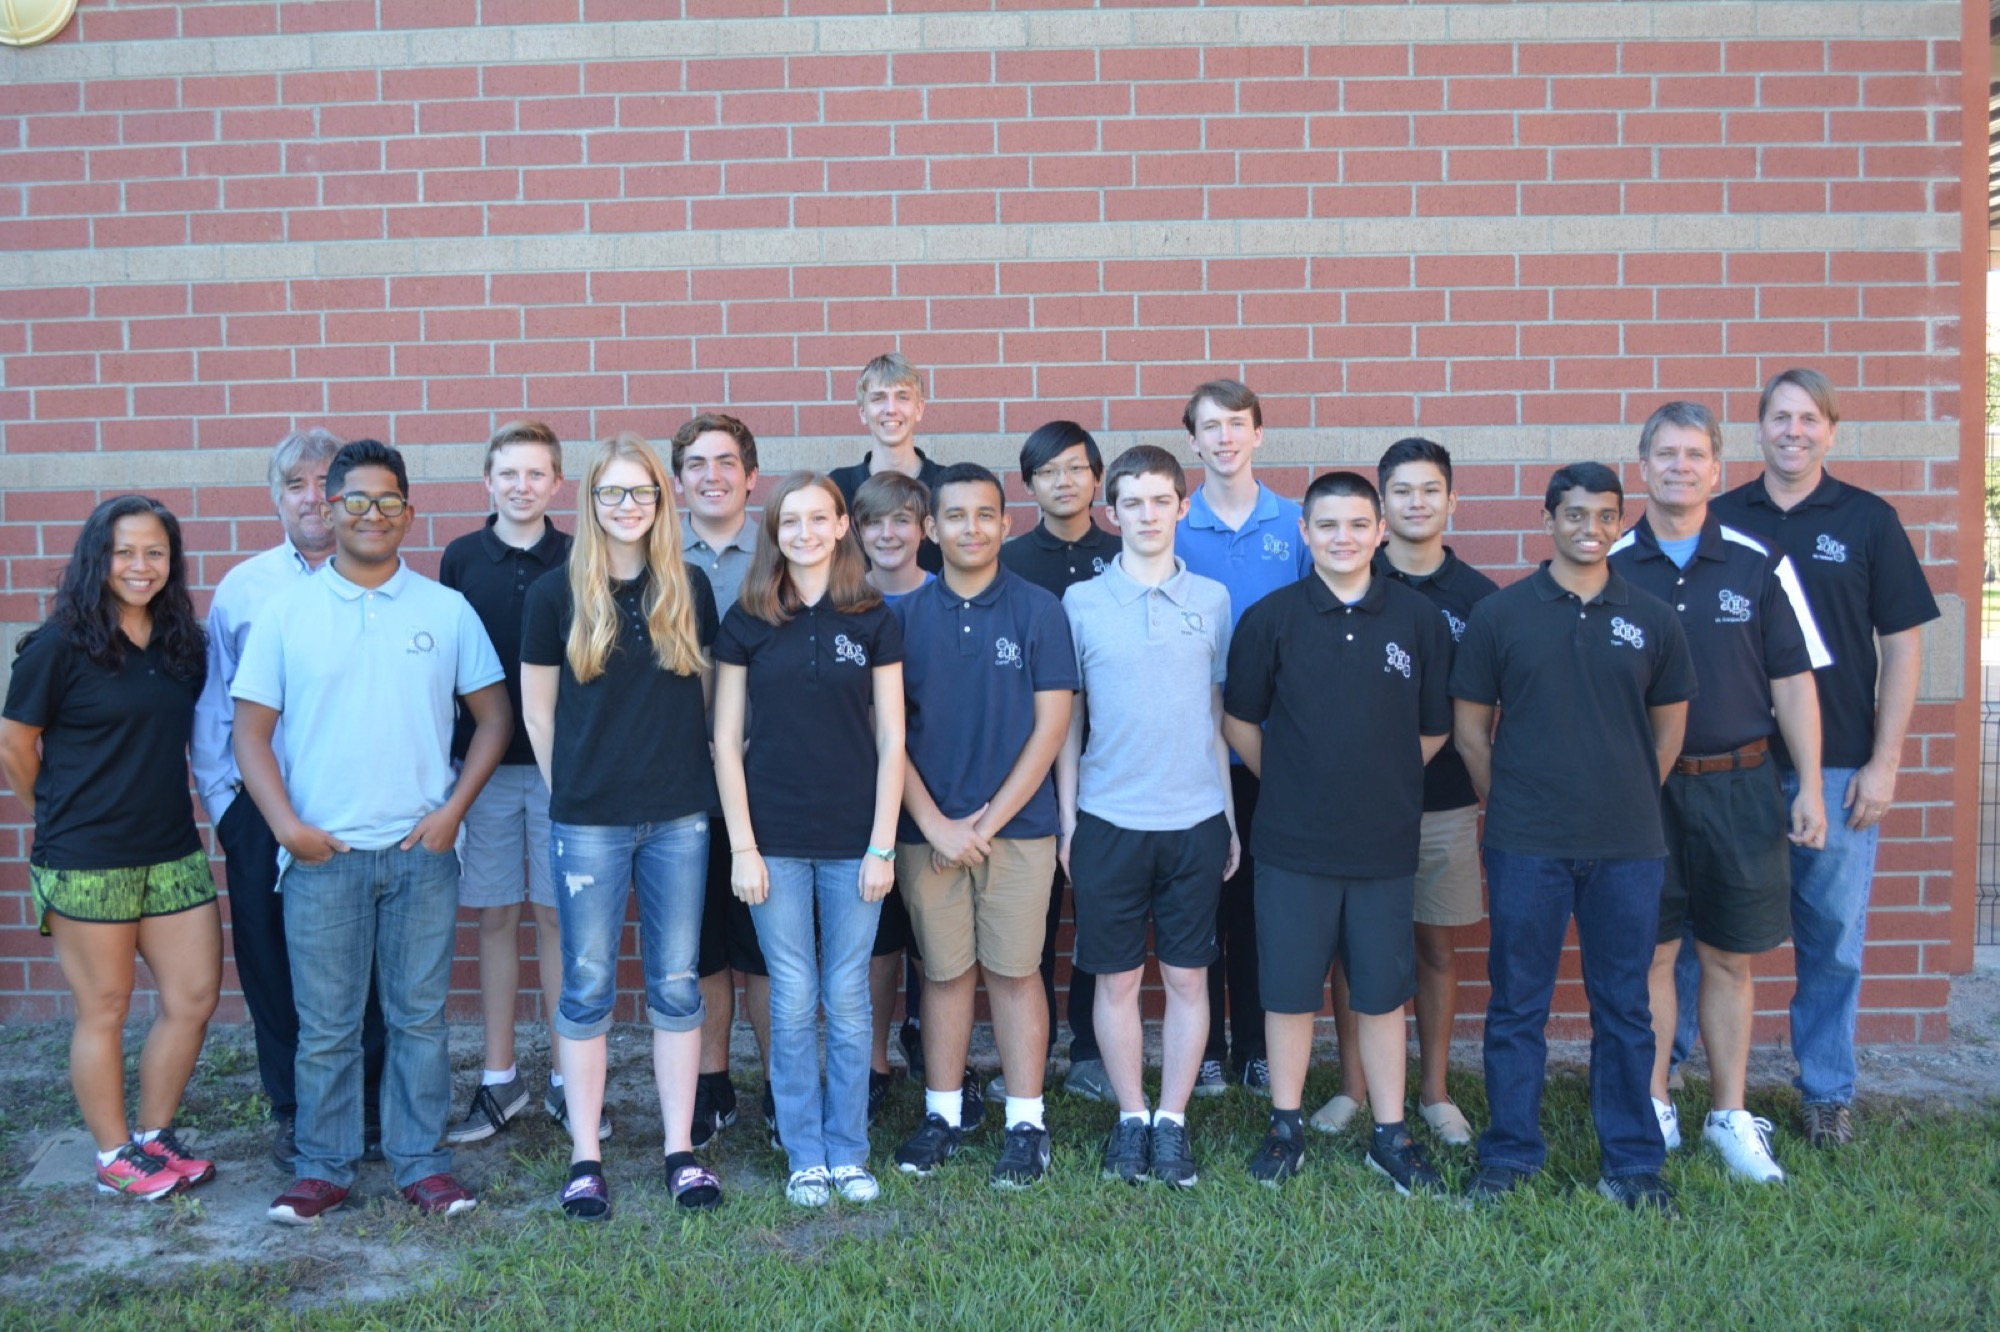
\includegraphics[width=0.8\textwidth]{Team4717.JPG}
% %\end{figure}

% \indent
% Within Hagerty High School, there lurks an atmosphere of surreptitious energy; the sounds of tinkering and hushed sibilation erupt in the dead of night, and shadowy hooded effigies loom around every corner. Who are these mysterious figures? These are the Mechromancers; they bring robots to life. Their codename: Team 4717. This team is undoubtedly a team full of effort, passion, and drive exemplified through their every action in the engineering process, outreach efforts, and competitive edge. The Mechromancers' main objective this year was to build a robot that was able to \hl{scale the crater, recover minerals, and shoot into the lander both quickly and accurately. Our robot's name this year is Bullseye, the second generation from the legendary Woody from 2016-17's Velocity Vortex.} We thought of keeping the Toy Story theme alive this year with having name of Bullseye be Woody's trusted steed, as well as being able to shoot with pin point accuracy.  

% \noindent
% \newline\textbf{\large Team Features:}
% \begin{itemize}
% 	\item \textbf{Extensive use of CAD} - Almost all parts of the robot were created in the Creo CAD software and built from raw materials. In Creo, movements are simulated using articulating joints, \textit{family tables} are used to create libraries of similar parts, \textit{skeletons} used for the top-down design, and all models are fully parameterized. \hl{Please view our design section, especially our page on the use of body and motion skeletons for the stabilization arms on page {\pageref{Stabilize:1}} to see an in-depth analysis on each mechanism in PTC Creo.}
%     \item \textbf{Outreach} - This year, our outreach team wanted to focus on promoting FIRST's values and the love for STEM and engineering in the community by making connections to other teams and our community in order to spread the values of FIRST and STEM. \hl{Refer to our Outreach Section to see our previous outreach events of this season, and learn about how we strive to build connections with businesses and organizations in our efforts to diffuse STEM across the world. For example, see how we founded and mentored an FLL Jr. Team on page {\pageref{FLLJR:1}}.}
%     \item \textbf{Organization} - We decided to keep our team organized through job specialization, breaking up into committees and subcommittees for each aspect of our team. This allows us to work in parallel while still working together. \hl{Check out our Committee Breakdown on page {\pageref{committees:1}} to learn about how the team is organized into these smaller committees, the role that each committee plays, and the members they consist of.}
%     \item \textbf{Custom Parts} - We used 3D printing as well as the laser cutter and machine shop at the University of Central Florida's Innovation Lab to create custom parts for the robot. \hl{Check out our Custom Parts Reference on page {\pageref{CustomPartsReference:1}} for the Creo sketch and CAD model of each part on our robot.} 
%     \item \textbf{Unique Notebook Format} - We use the \LaTeX typesetting language to create an engineering notebook that can be easily edited and formatted. We use Github to easily edit and share code.
%     \item \textbf{Always Evolving} - The Mechromancers are always yearning for innovative solutions to whatever issues we may face in competition, and therefore are always evolving. \hl{Refer to our Competition Section and our timeline on {\pageref{timeline:1}} to see how we evolved throughout the season.}
% \end{itemize} 

% \noindent \hl{Judges! Please be sure to check out the tabbed pages! We have included a description of the tabs in a table on the reverse side of this summary.} 

% Check out our robot \textit{Bullseye's} evolution through our design and build process in the upper right hand corner of each new meeting in the engineering section!
 
% \interestingpagetable 